\chapter{Analysis 2: Verbal Communication \& the Dakota Access Pipeline}
\lhead{\textit{Analysis 2: Verbal Communication \& the Dakota Access Pipeline}}

\textit{\textbf{Chapter Summary:} This chapter examines verbal communication (in the form of quotations from texts) in relation to the Dakota Access Pipeline. Segmenting speakers into three groups allows for comparative analysis showing how actors in the debate employ different keywords and connotations. Crucially, patterns of cultural discourse and stereotyping can be identified.}
\newline

\section{Background}

In August 2016, Indigenous protesters chained themselves to heavy machinery in North Dakota. In the following months, viewers worldwide saw protesters arrested, attack dogs unleashed, encampments bulldozed, and the heavily armed National Guard march in to the otherwise peaceful grasslands of Sioux County. At issue was the construction of the Dakota Access Pipeline, a \$3.8 billion project, proposed by the Dallas-based Fortune 500 company Energy Transfer Partners, which would transfer shale oil from the Northern Plains to the industrial heartland (Figure 4.1). The previous chapter approached the theme of GM seed through high level textual analysis. This chapter looks at a more localized environmental issue and by examining statements made by specific speakers. Here we are concerned with the debate surrounding the Dakota Access Pipeline as expressed in quotations by various stakeholders. 

Any analysis of communication surrounding the Dakota Access Pipeline (DAP) will have to account for diverse perspectives. Infrastructure and resource projects, as well as environmental issues in a broader sense, precipitate a complex dynamic of conflicting ideas, worldviews, and values. In the case of the DAP, this dynamic included spiritual values of the Native American Sioux; historical land disputes; issues of inequality and corporate power; science and engineering practice; local/national politics, and global environmentalism. 

For any project of this scale, there are voluminous communication artifacts one could analyze, ranging from court records and environmental assessments to news articles and social media posts. Having gained national and international headlines, the Dakota Access Pipeline resulted in an even greater volume of communication than is typical for such a project. As protests escalated through the fall months of 2016, the cause garnered support from outgoing President Obama and presidential candidate Bernie Sanders. Sioux leader David Archambault II brought the issue before the UN Human Rights Council in Geneva. This was followed by the UN Special Rapporteur on the rights of indigenous peoples calling for a halt to construction, stating that the Standing Rock Sioux tribe had been ``excluded from consultations'' \citep{OHCHR2016a}. In January 2017, as one of his first executive actions, the newly elected President Trump directed the U.S. Army Corps of Engineers to approve the pipeline in an ``expedited manner'' \citep{OfficeofthePressSecretary2017a}. Within weeks, authorities cleared out the last remaining protest camps and construction crews began drilling. By June, the oil was flowing. 

The protests drew international attention and reshaped the national conversation about resource projects on Native American land \citep{Liu2013a}. The fact that the protest site became the largest gathering of Native Americans in over 100 years \citep{Northcott2016a} puts the events in the context of deep and ongoing historical struggles for indigenous sovereignty and decolonization. 


\begin{figure}[H]
\centering
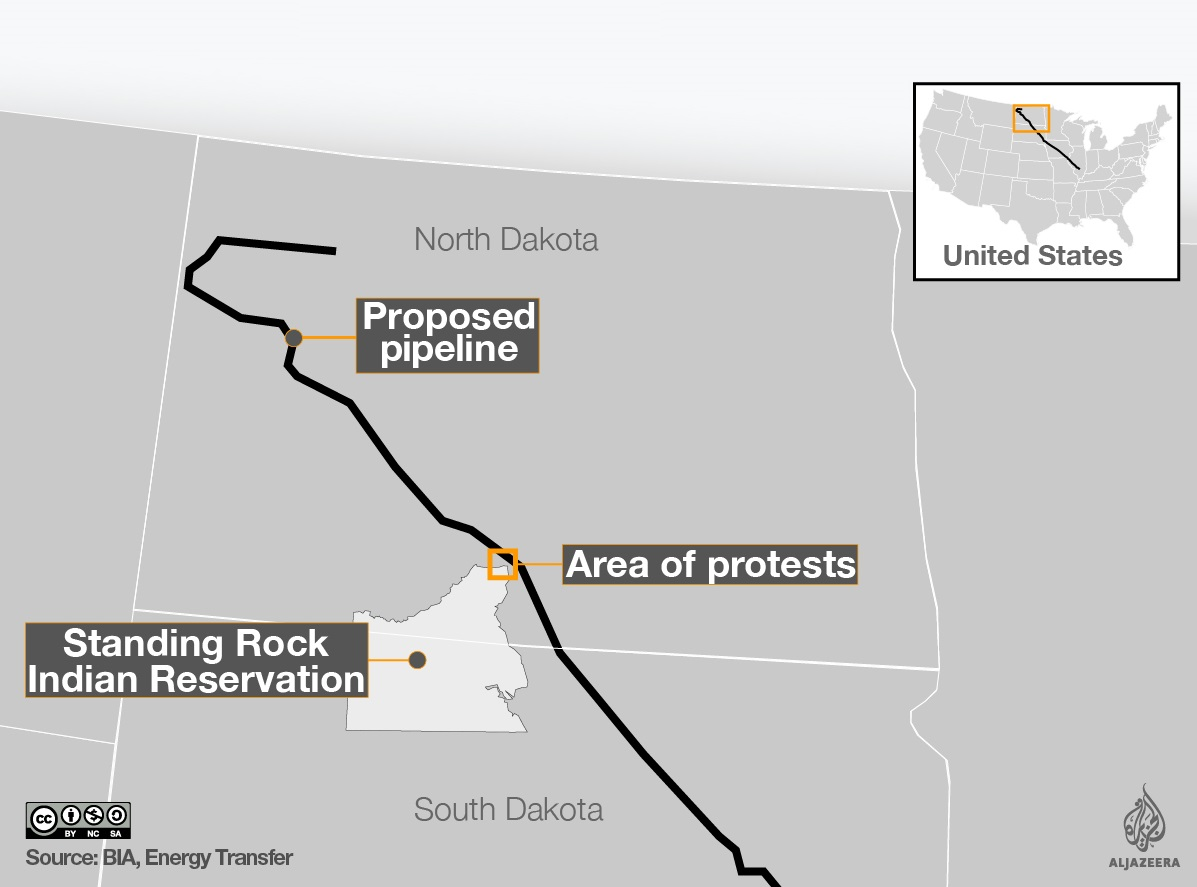
\includegraphics[width=9cm]{Figures/dakota.jpg}
\caption{Dakota Access Pipeline route}
\begin{footnotesize}
Creative Commons image from https://www.aljazeera.com
\end{footnotesize}
\label{fig:figure1}
\end{figure}

The challenge in describing communication surrounding this issue, is largely methodological. Disparate and voluminous data must be gathered and analyzed at a manageable scale, while also accounting for a breadth of sources and perspectives. Difficulties in scope and framing also become apparent when faced with methodological choices. At its core, one could argue, the pipeline is strictly a scientific and engineering problem. From another perspective, one could make the case that the issue is best approached in terms of power and class. Looking at discourse surrounding the issue also makes it clear that culture, specifically indigenous identity, is central to this issue. Even the time horizon is not entirely clear. Whereas the issue explicitly began in June 2014 (when the project was announced), one could also argue that it reaches back over 150 years ago with the Treaty of Traverse des Sioux (1851) and the Treaty of Fort Laramie (1868), when the U.S. Senate ratified treaties that recognized the Sioux peoples' national sovereignty. What follows is a multilevel framework for integrating the disparate aspects of the pipeline debate. 

\section{Corpus Data}

This second corpus corresponds to the verbal level and contains quotations related to the Dakota Access Pipeline. To build this corpus, quotations were collected from online articles. Granted, quotations from articles do not achieve the depth of primary sources and ethnographic interviews. However, there are several advantages of drawing from quotations in this way. Assuming that principles of responsible journalism were followed, quotations are accurate and reliable; they contain the original spoken words and editing will not have changed the meaning of statements \citep{CAJ2011a}. Collecting quotations also allows for large-scale data analysis and presentation of diverse perspectives.	

First, a corpus of articles was made by conducting an online search from two queries: ``Dakota Access Pipeline,'' ``Dakota Access pipeline AND protests.'' The result was 226 pages with a total word count of 300,000. Quotations were then extracted from the corpus using regular expression matching. 500 characters before and after each quotation were also extracted so, for each quote, the context as well as the speaker could be identified. 

The result was 628 quotations with contextual text snippets. After manual analysis, the list of 628 was reduced to 388 by balancing the speakers/perspectives and consolidating where there were several successive quotes by one speaker. A speaker was then assigned to each quotation, including a name as well as any other identifying information contained in the contextual snippets, such as occupation, origin, ethnicity, or institutional affiliation.

Once quotations were obtained, they were read (in context) and categorized according to the identities/stance of the speakers. Broadly speaking, speakers fell into one of three categories: (i) proponents of the pipeline; (ii) protesters/citizens directly opposing the pipeline; and (iii) people lending support for the cause of the protesters but not protesting in a direct manner. For the purposes of this analysis, the focus is on categories (i) and (ii), proponents and opponents. The quotations were then grouped according to the stance of the speakers as well as context of the statements (Figure 4.2). Quotes from proponents (i.e. quotes made in the context of advocating for the pipeline or denouncing the protesters) were put into Group A. Groups B and C both contain quotes from pipeline opponents/protesters. Group B contains quotes that related to rights, justice, and equality. Group C is reserved for quotes more explicitly expressing culture and identity.  

\begin{itemize}
  \item \textbf{Group A}: Proponents who either actively voiced support for the pipeline (e.g. company representatives) or took a legal or institutional stand against the pipeline protesters (e.g. law enforcement)
  \item \textbf{Group B}: Protesters/opponents raising issues of trust, fairness, or inequality (e.g. rights to land, oppression of law enforcement)
  \item \textbf{Group C}: Protesters/opponents expressing cultural identity, such as group membership or cultural assertions (e.g. values, worldviews, ethnic/linguistic identity)
\end{itemize}

\begin{figure}[H]
\centering
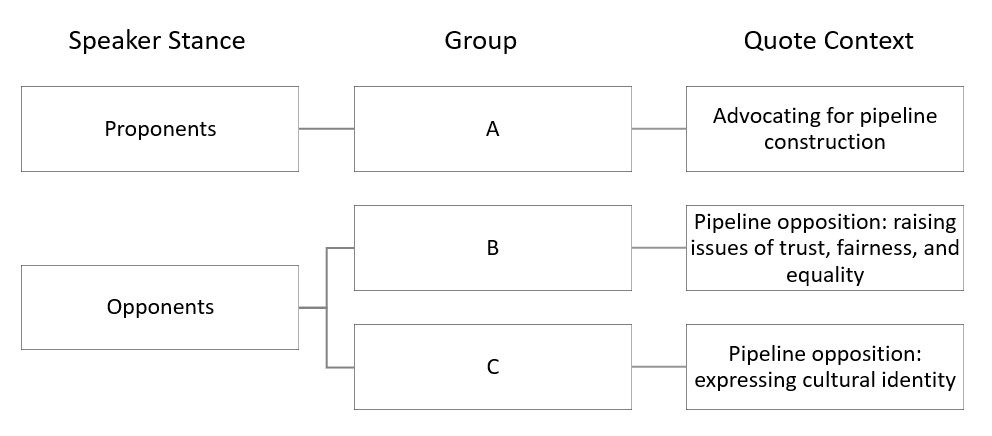
\includegraphics[width=13cm]{Figures/groups.png}
\caption{Groupings of quotations}
\label{fig:figure1}
\end{figure}

\section{Multilevel Analysis}

Multilevel analysis can help us understand a complex topic like the DAP. The issue is obviously and, perhaps most explicitly, ecological. The cultural aspects of the DAP are also explicitly expressed by the indigenous stakeholders. However, the data suggest socio-economic factors also pervade the issue, albeit these factors are often expressed more indirectly in comparison with the ecological and cultural levels.

Compared to Analysis 1, this analysis relies on more manual and qualitative methods. Focusing on quotations allows for this manual analysis, since the corpus is reduced to a manageable size. Most importantly, focusing on quotations is a way to associate specific statements with specific speakers and their identities\textemdash something that would not be possible with the corpus in the previous chapter (Analysis 1).  

At the level of verbal quotations, the overlap between the different levels of analysis becomes apparent. In other words, it becomes clear that the ecological, cultural, socio-economic, and cognitive levels are not distinct categories. In fact, one single statement might span all or several of these levels. However, categorizing and grouping the quotations is a way to clarify the levels and their interrelation.

One might question the decision to separate a subset of quotations as `cultural'. The implication, of course, is that certain statements are not cultural, contradicting the notion that culture is everywhere and pervasive is all human communication. However, based on the distinction (from Chapter 2) between culture and civilization, we are proposing that some utterances are, indeed, more cultural than others. For instance, we see that, in comparison with Group C, Group A does not contain cultural meanings such as personhood, relationships, or identity.

\textbf{Keyword Analysis}

Keyword analysis points to dominant themes in each group. Quotes were processed by removing punctuation, cases, symbols, and stop words as well as performing stemming and lemmatization. For each of the 3 groups, the top 20 keywords were then obtained based on frequency (Table 4.1).  

Keywords in Group A such as \textit{law}, \textit{state}, \textit{federal}, \textit{company}, and \textit{police} are indicative of discourse related to institutions. It is also relevant to note that \textit{protester} is the second most common term in Group A, whereas it does not appear in the other groups. A possible explanation is that \textit{protester}, with pejorative undertones, is part of identity construction and `othering' rather than a term people use to describe themselves. The terms \textit{behavior}, \textit{aggressive}, and \textit{safety} also point towards possible negative portrayals of citizens opposing the pipeline. Finally, it might be noted that the only apparent environmentally-related term in Group A is \textit{energy}, which is a dominant theme of the pro-pipeline side (i.e. \textit{energy} independence, \textit{energy} infrastructure, \textit{energy} security).  

In Group B keywords, cultural language begins to emerge with \textit{nation}, \textit{indigenous}, or \textit{Dakota}. Through \textit{right}, \textit{government}, and perhaps \textit{force}, one can see evidence of the rights-based or anti-oppression discourse. This is expected since the category contains quotes related to issues of trust, fairness, and equality. The keywords \textit{land} and \textit{water} indicate the ecological thrust of this group, whereas the absence of \textit{energy} contrasts with that of Group A. Group C keywords bring the cultural themes into more focus. Along with \textit{indigenous}, this group features the words \textit{prayer}, \textit{sacred}, and \textit{human}. In addition to \textit{water}, the ecological-related keywords in Group C include \textit{earth} and \textit{life}.   

\begin{table}[H]
\begin{footnotesize}
\centering
\begin{tabular}{|l|l|l|l|l|l|}

\hline
\multicolumn{2}{|l|}{\textbf{Group A}}           & \multicolumn{2}{l|}{\textbf{Group B}}            & \multicolumn{2}{l|}{\textbf{Group C}}            \\ \hline
\textit{\textbf{Word}} & \textit{\textbf{Freq.}} & \textit{\textbf{Word}} & \textit{\textbf{Freq.}} & \textit{\textbf{Word}} & \textit{\textbf{Freq.}} \\ \hline
pipeline              & 5                       & people                 & 9                       & people                 & 13                      \\ \hline
protester                 & 4                       & nation                 & 6                       & going                  & 10                      \\ \hline
energy                    & 4                       & iowa                   & 6                       & camp                   & 8                       \\ \hline
law                  & 4                       & indigenous             & 5                       & water                  & 7                       \\ \hline
state               & 3                       & dakota                 & 5                       & protect                & 7                       \\ \hline
transfer                & 3                       & government             & 5                       & pipeline               & 6                       \\ \hline
partner                & 3                       & right                  & 5                       & prayer                 & 6                       \\ \hline
federal                 & 3                       & water                  & 4                       & right                  & 6                       \\ \hline
people                  & 3                       & project                & 4                       & something              & 6                       \\ \hline
think                 & 3                       & going                  & 4                       & fight                  & 5                       \\ \hline
others                & 3                       & land                   & 4                       & life                   & 5                       \\ \hline
company               & 3                       & trying                 & 3                       & indigenous             & 5                       \\ \hline
behavior                 & 2                       & would                  & 3                       & future                 & 5                       \\ \hline
safety                 & 2                       & say                    & 3                       & sacred                 & 4                       \\ \hline
caused                 & 2                       & industry               & 3                       & think                  & 4                       \\ \hline
police                   & 2                       & get                    & 3                       & human                  & 4                       \\ \hline
said             & 2                       & far                    & 3                       & need                   & 4                       \\ \hline
aggressive                  & 2                       & pipe                   & 3                       & mother                 & 4                       \\ \hline
would                 & 2                       & force                  & 3                       & earth                  & 4                       \\ \hline

\end{tabular}

\caption{Keywords from each group of quotations}
\label{tab:table1}
\end{footnotesize}
\end{table}

\subsection{Ecological Level}

Picking up on the keyword analysis, this section looks closer at the ecological themes in the quotations. The environmental debate surrounding the Dakota Access Pipeline spans local, national, and global dimensions. Pipeline opponents allege the pipeline's crossing of the Missouri River constitutes a threat to the region's clean water. However, more global issues, notably climate change, are also key motivations for resistance. Project proponents, on the other hand, often cite the relative safety of pipeline transport vis-\`a-vis the alternatives. The theme of national energy independence and energy security is also advanced by proponents. 

It is important to note that, although the pipeline is clearly a topic of environmental debate, ecological topics are not central to the quotations. In Group A, for instance, there are 23 quotations and only 2-3 explicitly address the environmental issues. 

In addition to direct ecological-level considerations, this section discusses the relation between environmental issues and other themes in the discourse. As in Analysis 1, we consider how the environment is framed. The quotations give indications of how the natural world is construed by different actors. 

\textbf{Group A: Discourse of Security}

In Group A, the environment is framed through projects and infrastructure. The natural world is spoken of in terms of resources and management. Consider the following statements by the company proposing the project.

\begin{footnotesize}
\begin{itemize}
\item[] \texttt{[We] developed response and action plans, and will include several monitoring systems, shut-off valves, and other safety features to minimize the risk of spills....\newline \textit{-Energy Transfer Partners spokesperson}} 
\newline
\item[] \texttt{[the project meets] all applicable federal, state and local environmental laws, regulations and standards.... We continually seek ways to enhance our operations in the areas of environmental and resource protection and conservation.\newline \textit{-Energy Transfer Partners spokesperson}} 

\end{itemize}
\end{footnotesize}

The first statement frames the physical environment as something that can be managed and controlled through technology. The second statement also refers to management, albeit in the context of laws and regulations as opposed to technology. Both statements refer to the natural world through human intermediaries and institutions. No doubt, they are intended to convey an impression of competence and control with respect to the built, physical environment.

Aside from statements about managing risks, proponents also make the case for the pipeline as needed energy infrastructure. The following statement from Group A typifies this position:

\begin{footnotesize}
\begin{itemize}
\item[] \texttt{We think this is a great step forward for energy security in America.\newline \textit{-President of the North Dakota Petroleum Council}}
\end{itemize}
\end{footnotesize}

This quote indicates the national geographical focus (i.e. \textit{America}) that is common in the proponents' discourse. While the opposition discourse also has national references, the focus is on local/regional environmental impacts (e.g. risk of water contamination) as well as the global-level (e.g, climate change). Although local jobs are also a factor, the project being in the national interest is a key argument among proponents.  

The word \textit{security} is notable in the quote above. As the keywords indicate, \textit{security} (in the sense of law and order) is a reoccurring theme in Group A. In the quote above and in the text data as a whole, we see this theme extends to the ecological realm with the notion of \textit{energy security}. This suggests that discourses of public safety and national security are intertwined with those of environmental and resource security. In both cases, there is a perceived threat (e.g, energy insecurity, dependence) together with a set of actions to confront that threat. 

From a discourse analysis perspective we might also consider how \textit{security} functions in order to justify and legitimize certain actions that may be outside of the norm. For example, using a corpus of documents from security organizations, \cite{MacDonald2019} posit that \textit{security} functions to construct a state of exception while (seemingly) adhering to liberal-democratic principles. Likewise, the notion of \textit{energy security} might mobilize a discourse whereby the pragmatic ends of national interest and cheap energy are used to counter environmental concerns. In other words, if environmentalism itself creates a state of exception (e.g. to justify civil disobedience), the discourse of \textit{security} is a response that invokes economic and national interest.

\textbf{Group B: Discourse of Environmental Justice}

Insofar as quotations in Group B concern the ecological-level, they are often more political in nature. For instance, a number of speakers address the perceived conflict of interest among regulators and the oil and gas industry. At this ecological-level of analysis, we note how the environment emerges as the cite of political/economic injustice. In particular, infrastructure is seen as reflecting power dynamics of the broader society and resisting projects is a way to resist perceived injustices in those dynamics. The following quotes reflect this sentiment:  

\begin{footnotesize}
\begin{itemize}
\item[] \texttt{North Dakota regulators are really, I would say, in bed with the oil industry and so they have looked the other way.\newline
\textit{-Winona LaDuke, Ojibwe activist and Green Party candidate}}
\newline
\item[] \texttt{...big business and big ag are pulling the levers of government in Iowa.
\newline
\textit{-Adam Mason, Iowa Citizens for Community Improvement}}
\end{itemize}
\end{footnotesize}

Similarly, consider the following quote by a citizen who came to the protests from Flint, Michigan. The speaker is referring to the \textit{Flint water crisis} where, due to mismanagement by regulators and cost-cutting measures, drinking water was contaminated in the city of Flint.\footnote{The Flint water crisis started in 2014 when officials failed to apply corrosion inhibitors to the water. As a result, lead from aging pipes leached into the water supply, exposing over 100,000 Flint, Michigan residents to elevated lead levels.} 

\begin{footnotesize}
\begin{itemize}
\item[] \texttt{We know in Flint that water is in dire need,... In North Dakota, they're trying to force pipes on people. We're trying to get pipes in Flint for safe water.}
\end{itemize}
\end{footnotesize}

Whereas Group A clearly contains statements intended to convey management competency and legitimacy over natural resources, statements from Group B challenge the legitimacy of regulators and industry. Given these themes, Group B is discussed in more detail in the later socio-economic level of analysis. The crucial point here, however, is that speakers in Groups A and B form a coherent discourse between them, at least with respect to ecology and environment. In other words, there is an extent to which the discourses of Groups A and B are in dialogue with each other. The points made by each side have a common context and framework for meaning. The language is that of legitimacy/governance over resources and infrastructure. By contrast, in the next section we consider how, in Group C, ecological language is part of an entirely different framework of meaning.  

\textbf{Group C: Environment and Cultural Identity}

In Group C, references to the natural world are made in the context of cultural identity, values, and human well-being. In various quotes, the notion of culture is emergent in the sense that it results from the interplay of different elements, including the natural world. In contrast to Groups A and B, the environment is not framed through infrastructure and resources; rather, it takes on a more intrinsic value. There is a notable contrast with Group A where there is an analytical approach to the environment as something to be managed. Group C, by contrast, contains more holistic views of relationships and interactions with the environment. The following quote is an example: 

\begin{footnotesize}
\begin{itemize}
\item[] \texttt{We are going to keep it going, keep organizing meetings and find a way to be able to take care of the health and welfare of our people, and preserve land and water.   \newline
\textit{-Ivan Lookinghorse, Cheyenne River Reservation}}
\end{itemize}
\end{footnotesize}

By juxtaposing health and welfare with ecological preservation (as opposed to speaking in strict cause and effect terms), the speaker invokes a complex set of relationships and interactions. Here, the cause and effect relationship between the environment and human health is present, but the case for ecological preservation is not reducible to human health. In other words, there is cultural value\textemdash as opposed to strictly utility value \textemdash placed on preservation. The following quote also points to complex interactions between the environment and the economic, political, and cultural spheres:

\begin{footnotesize}
\begin{itemize}
\item[] \texttt{...in peaceful prayer and in dignity as we assert our rights to protect our environment, our economy and our sovereignty.   \newline
\textit{-Chase Iron Eyes, activist}}
\end{itemize}
\end{footnotesize}

The possessive pronoun \textit{our} clearly indicates the speaker is invoking cultural identity. Crucially, this identity entails a holistic relationship between the environment and economy. Contrast this with Group A, where the national economy (i.e. energy security and national interest) is invoked to defend pipeline construction. The emphasis on relationships is also apparent in following quote: 

\begin{footnotesize}
\begin{itemize}
\item[] \texttt{We're here today to send a message that we, as human beings, are indigenous to the earth. The earth is our mother. Your relationship with the mother is forever. The earth gives us our water, our air, our food, our shelter. We need to protect it.  \newline
\textit{-Cassandra Begay, a member of the Navajo tribe}}
\end{itemize}
\end{footnotesize}

This is one of a number of quotations in Group C that use personification of earth as \text{mother} as an embodiment of life-giving and nurturing aspects of nature. Even though the last part of the example (``The earth gives....'') could be said to refer to the utility value of nature, the \textit{mother} metaphor frames nature in a way that transcends any means-ends, utilitarian representations. 

As in Analysis 1, depending on the context, we see stark contrasts between the way in which nature is referred to. In Group A, nature is framed in a physical, commodity-based manner. Speakers reference management of specific systems of infrastructure and materials as opposed to holistic interactions and intrinsic value. Group B maintains this framing, insofar as speakers are challenging the legitimacy to jurisdiction over materials and energy. 

In Group C, nature is takes on an entirely different frame of meaning. It is part of holistic relationships and interactions with people, culture, and the economy. It is in this sense that speakers in Group C are communicating within an entirely different framework that integrates layers of meaning, including cultural/spiritual expression. 
  
\subsection{Cultural Level}
Indigenous communities are, of course, the predominant cultural groups affected by the pipeline and involved in the protests. A key question, then, is how the discourse is reflective of these communities, or how analogous observations apply to other identifiable groups. Of course, this presupposes that we can indeed identify speakers as members of distinct groups. In other words, we first need to inquire as to how group identities are expressed and constructed. 

Distinguishing between cultural groups or speech communities carries the risk of essentializing identities \citep{Dervin2016a, Piller2007a} or stereotyping `the other' \citep{Fedor2014a}. At the same time, these very group identities are also rich, meaningful aspects of experience and selfhood. It is important, therefore, to distinguish between instances where speakers identify themselves as members of cultural groups versus instances where an identity is assigned/constructed by others in the society. The present analysis looks at cultural identities that are explicitly expressed by speakers. In other words, we are interested in cultural indicators in communication, such as group membership, pronoun usage, or other markers of identity. 

We can also distinguish between expressions of self identify versus cases where an identity is assigned/constructed. In other words, of interest are both self expression of identities (e.g. ``\textit{we} are indigenous'') as well as cases where identities are applied to others (e.g. ``\textit{they} are eco-terrorists''). The latter often involves othering. Othering involves defining a person or group in a negative way that creates distance and difference \citep{Powell2017}. Here we argue that othering is a process of stripping away culture; it is the antithesis of intercultural communication in the sense that a cultural group is labelled or outright denied, rather than understood in familiar terms.  

\textbf{Othering as Negation of Culture}

In the source quotations, the theme of culture does not occur until groups B or C. Cultural groups are scarcely mentioned in Group A. One could question the overall significance of the absence of culture in Group A, and the degree to which this absence is an intended feature of discourse of pipeline proponents. 

Rather than through cultural identity, speakers in Group A refer to protesters in the negative terms of othering. Consider the following segments from Group A:

\begin{footnotesize}
\begin{itemize}
\item[-] \texttt{Protesters' escalated unlawful behavior}
\item[-] \texttt{[protesters had been] very aggressive}
\item[-] \texttt{eco-terrorist groups}
\item[-] \texttt{the anti-DAPL diaspora}
\item[-] \texttt{these things can be overwhelmed from outside groups}
\item[-] \texttt{a large component is very violent, very confrontational}
\item[-] \texttt{There is an element there of people protesting who are frightening. It's time for them to go home.}
\end{itemize}
\end{footnotesize}

Rather than referring to the protesters as identifiable people, they are anonymized as ``protesters'' or ``groups.'' Despite the fact that the protest camp was established by local Standing Rock Sioux tribal citizens, statements by pipeline proponents scarcely mention this group or other indigenous communities. In fact, phrases such as ``diaspora'' or ``outside groups'' create the image of geographically dispersed individuals with no local ties or history. In addition, protesters are characterized as ``unlawful,'' ``aggressive,'' ``violent,'' ``confrontational,'' and ``frightening.'' These adjectives disassociate protesters from society. Crucially, this disassociation is not made through cultural difference. Instead, it coincides with the rendering of protesters as an anonymized mass of individuals as opposed to culturally identifiable groups.

By contrast, in groups B and C, speakers refer to themselves in culturally identifiable terms as indigenous people or by using the words ``we'' or ``our.'' Consider these segments from groups B and C: 

\begin{footnotesize}

\textbf{Group B}

\begin{itemize}
\item[-] \texttt{We don't ever hear the narrative of indigenous people.  We hear people writing our narratives for us.}
\item[-] \texttt{We are suffering the highest rates of cancer}
\item[-] \texttt{treating the original inhabitants of this land as though we are less than human}
\item[-] \texttt{Our people are continuously brushed aside for an industry advancement that will only line the pockets of the top 1 percent.}

\end{itemize}
\end{footnotesize}
\begin{footnotesize}
\textbf{Group C}
\begin{itemize}
\item[-] \texttt{our treaty rights and risk our water}
\item[-] \texttt{we were invisible people}
\item[-] \texttt{We will continue to provide for our people}
\item[-] \texttt{When we have ceremonies, we do camps like this. It's something that we've always known how to do, going back to pre-colonial times.... irreparable harm for us in our culture.}
\item[-] \texttt{As Indian people, we have a right to protect our lands and protect our water we that live here have to deal with racism or prejudice more now than before.}
\end{itemize}
\end{footnotesize}

The distinction between B and C is analogous to that in the ecological-level, where B is a reaction to A and C is culturally affirmative. Although statements in Group B assert group identity, it is in reaction to social structures. For instance, Group B refers to marginalization, negative health outcomes, racism, discrimination, and inequality. In Group C, speakers assert group identities based on social bonds, shared history, ceremonies, and relationship to place. 
The above groupings show that the very notion of cultural identity is undermined in the discourse. Group A statements strip away or evade the cultural context. This is problematic insofar as it is a barrier to mutual understanding. Based on the notion that cultures are family resemblance concepts \citep[10-11]{Frayne2017a}, we come to understand unfamiliar practices and beliefs through analogy to, and likeness of, those more familiar. The basis for such comparison are shared, human forms of life that cut across identities. Othering effectively diminishes the capacity to recognize this shared basis by creating distance and defining people in negative terms. 

\textbf{Cultural Discourse in Affirmative Terms }

The implication of the previous groupings is that cultural analysis applies mainly to a subset of the discourse. It should come as no surprise that, among all the quotations, those which do lend themselves to cultural analysis are found in Group C. Looking closer at this group allows us to characterize cultural discourse in the affirmative, as opposed to in negative terms (i.e. that which a group is opposed to). For example, in Group A, we see examples of unity and reciprocity between different people. 

\begin{footnotesize}
\textbf{Group C}
\begin{itemize}
\item[-] \texttt{People have been surviving here for hundreds and hundreds of years...so if I back down, what would I look like?}
\item[-] \texttt{...spiritual battle.... This is a protest about the stewardship of God's creation and justice for the indigenous peoples of the Great Plains}
\item[-] \texttt{The idea of small-is-beautiful is important here I think.... This was an ethic popularized by the American counterculture but quickly adopted by indigenous peoples globally as a means of reconciling nature, culture and technology.}
\item[-] \texttt{But keep the coalitions together, because there are more pipelines proposed, and we must protect our Mother Earth for our future generations.}
\item[-] \texttt{As Indian people, we have a right to protect our lands and protect our water we that live here have to deal with racism or prejudice more now than before}
\item[-] \texttt{We've recognized that human spirit within each other. Because that human spirit doesn't have a color.}
\end{itemize}
\end{footnotesize}

In the above segments, speakers refer to shared values and common themes. For instance, spirituality and a sense of the sacred is clearly a cross-cutting theme. Although statements such as ``stewardship of God's creation'' may come from a different theological perspective than other expressions of the sacred, the speaker is drawing from commonalities (e.g. the natural environment as endowed with spiritual significance) rather than the differences (e.g. Christian vis-\`a-vis other spiritual traditions). Shared principles and values also serve as common ground. Pride, compassion, and ``the human spirit'' are mentioned as unifying factors among diverse groups, as is exemplified by the statement ``human spirit doesn't have a color.''

\subsection{Socio-Economic Level}

The ecological-analysis above shows how proponent (Group A) statements aim to uphold the claim of legitimacy that certain actors (i.e. companies, regulators) assert over natural resources and infrastructure. In turn, in the cultural analysis, we see how othering seeks to reinforce this legitimacy by characterizing pipeline opponents in negative terms. The present socio-economic analysis expands on the themes of legitimacy and othering, with a focus on how cultural identity and othering intertwines with socio-economic structures.

\textbf{Omission of Differences}

Along the same lines as othering, we also see the omission of differences, whereby group differences are not mentioned. Consider the following quotes from Group A and Group B, respectively: 

\begin{footnotesize}
\begin{itemize}
\item[] \texttt{We are very pleased to bring this important infrastructure project that benefits all Americans and our national economy into service on June 1.\newline \textit{-Lisa Dillinger, Energy Transfer spokeswoman}}
\newline
\item[] \texttt{The U.S. must recognize that we have political equality.  This is much larger than a specific infrastructure project. It goes to the fundamental relationship.\newline \textit{-Fawn Sharp, Quinault Indian Nation and the Affiliated Tribes of Northwest Indians}}
\end{itemize}
\end{footnotesize}

While the first quote positions the pipeline in terms of the ``national economy'' for ``all Americans,'' the second takes exception by suggesting there are some groups, namely indigenous peoples, who either do not benefit or are harmed by the pipeline. The second quote is part of a discursive space based on a plurality of relationships between diverse actors. The first quote, however, undermines these distinctions and relations, by folding the body politic into a mass of ``all Americans.''

In fact, the quotations in Group A scarcely mention cultural groups and other segments of the population. Quotes mention ``the people of North Dakota,'' ``energy security in America,'' and ``this country,'' but do not get more specific about the distinct groups opposing the pipeline. These omissions might be seen as part of othering. While distancing the protesters as anonymized ``groups,'' the discourse simultaneously gathers all people together under national and state identities. 

\textbf{Economics Over the Public Sphere}

By omitting group identities, the Group A discourse appeals to a utilitarian reasoning where the pipeline is positioned as a benefit for the mass population. This gives way to discourse where economics and private interests are paramount over citizenship and the public sphere.

Consider the following Group A segments responding to the Obama Administration's pulling of its previously issued permit for the Dakota Access pipeline:

\begin{footnotesize}
\begin{itemize}
\item[] \texttt{...political interference...further delay in the consideration of this case would add millions of dollars more each month in costs which cannot be recovered.\newline 
\textit{-Energy Transfer Partners}}
\newline
\item[] \texttt{This action is motivated purely by politics at the expense of a company that has done nothing but play by the rules it was given. \newline   
\textit{-Energy Transfer Partners CEO, Kelcy Warren}}
\newline
\item[] \texttt{Today's unfortunate decision sends a very chilling signal to others who want to build infrastructure in this country.\newline    
\textit{-Kevin Cramer, U.S. House of Representatives}}
\end{itemize}
\end{footnotesize}

In the first quote above, the term ``political interference'' is used alongside a reference to how much construction delays would cost. The second quote ``motivated by politics'' is followed by reference to the law abiding nature of the company. In both cases, politics is used in a pejorative sense. An underlying ideological assumption is that the role of governance is to promote private economic interests. The third quotation has a similar effect, suggesting that the decision will deter future infrastructure investment.  

Although the quotes above are expected reactions to the situation, they point to the extent to which modern public discourse is the jockeying of private interests. If the public sphere as a space for common action and deliberation among a plurality of citizens, the quotes above are indicative of discourse that closes off the public sphere and puts private (economic) interests ahead of public deliberation. 

As argued above, Group A omits and negates distinct, identifiable groups. This amounts to an omission of the entire public discourse of these groups. Rather than deliberate with groups, statements in Group A evade genuinely \textit{public} discourse altogether, in favour of private pursuits.   

\textbf{Legitimacy and Institutional Trust}

In Group B we see critiques of social, political, and economic structures. As discussed earlier, Group B can be seen as a reaction to the legitimacy of proponent actors and institutions, such as state institutions and corporate entities. Here, we consider the various expressions of inequality and injustice. Apparent in Group B are the many targets of these expressions: ranging from law enforcement, media, historical injustice, racism, and economic inequality.

A sense of abuse of power and overreach on behalf of state law enforcement is widespread in Group B. The following quotes are just some of the many expressing these sentiments:

\begin{footnotesize}
\begin{itemize}
\item[] \texttt{The cops watched the whole thing from up on the hills. It felt like they were trying to provoke us into being violent when we're peaceful.\newline 
\textit{-woman protester (unnamed)}}
\newline
\item[] \texttt{Confronting men, women, and children while outfitted in gear more suited for the battlefield is a disproportionate response. \newline   
\textit{-David Archambault II,  tribal chairman, Standing Rock Indian Reservation }}
\newline
\item[] \texttt{[my daughter was] strip-searched in front of multiple male officers, then left for hours in her cell, naked and freezing.\newline    
\textit{-Brave Bull Allard }}
\newline
\item[] \texttt{It is because of the behavior of the state that these tensions are heightened.\newline    
\textit{-David Archambault II}}
\end{itemize}
\end{footnotesize}

Contrast the quotes above with those in Group A which discuss law enforcement and security. Recall that in Group A, protesters are characterized as ``unlawful,'' ``aggressive,'' ``violent,'' ``confrontational,'' and ``frightening.'' The statements above, by contrast, portray law enforcement as aggressors and instigators. In addition to unwarranted use of force, the quotes above raise concerns about due process and the rule of law. 

Statements about law enforcement relate to specific actions at the protest site. In Group B we also find expressions of systemic injustice. In other words, the critique and challenge to legitimacy is more far reaching than events surrounding the protests. For example, the quotes below raise issues of media representation. 

\begin{footnotesize}
\begin{itemize}
\item[] \texttt{It's just been escalating to that point where we have to use our phones to just show our side of our story. \newline 
\textit{-protester E'sha Hoferer}}
\newline
\item[] \texttt{We don't ever hear the narrative of indigenous people.  We hear people writing our narratives for us.\newline   
\textit{-Eryn Wise, Council communications director}}
\end{itemize}
\end{footnotesize}

The first quote refers to a perceived failure on behalf of mainstream media outlets to convey the message of pipeline protesters and, as a result, the need to use social media and first hand recordings of events. The second is a broader expression about not only media representation, but all portrayals of indigenous people. This second quote is crucial because it is apparent the issue is about more than the events surrounding the protest camps. In other words, the pipeline is understood as part of boarder forces of exclusion and injustice.

Along the same lines, the following statements refer to the historical relationship between the state and indigenous people in America:  
  
\begin{footnotesize}
\begin{itemize}
\item[] \texttt{Trump's reversal of that decision continues a historic pattern of broken promises to Indian tribes and violation of treaty rights. They will be held accountable in court. \newline 
\textit{-Jan Hasselman, lead attorney for the Cheyenne River Sioux tribe}}
\newline 
\item[] \texttt{[we call upon President Barack Obama to communicate] nation to nation, as indicated by our treaties. \newline 
\textit{-Chief Arvol Looking Horse, Cheyenne River Reservation in South Dakota}}
\end{itemize}
\end{footnotesize}  
  
These quotes refer to the historical relationship and, in the case of the first quote, cite a history of broken treaties. However, in both statements, an appeal is made to the rule of law and state institutions to restore and uphold the relationship with indigenous peoples. In other words, there is a degree of belief that prevailing legal and political mechanisms can address the issue. This position may be influenced by the fact that the speakers are both acting in an official capacity, the first as a legal professional and the other within a legally recognized system of government. In short, these quotations invoke the historical injustice but do not seriously challenge the legitimacy of the state.

By contrast, in other quotations, institutional legitimacy is not granted. Speakers display less trust that institutions will conduct themselves in a manner that is in the best interest of citizens. Consider the following quotes:

\begin{footnotesize}
\begin{itemize}
\item[] \texttt{...we have no faith in the Iowa Utilities Board or Dakota Access.  \newline 
\textit{-Matt Ohloff, Iowa Citizens for Community Improvement}}
\newline 
\item[] \texttt{We do not trust the government, period. \newline 
\textit{-Michael Her Many Horses, Lakota historian}}
\end{itemize}
\end{footnotesize}  

These statements are quite different from the previous two with respect to the lack of trust they display. Whereas the previous quotes display a willingness and desire to engage with institutions, these quotes dismiss the legitimacy of the institutions altogether. One possible justification for the difference is that the speakers are different. Compared to the first two quotes from a lawyer and tribe Chief, these are spoken by people acting in more unofficial capacities (a member of a citizens group and historian, respectively). Accordingly, one might expect the latter speakers to be more unrestrained in their language and, perhaps, more closely reflect the views of citizens/protesters at large.

A further level of social distrust is related to economic inequality. The following quotes show how speakers in Group B link the pipeline to economic factors and wealth distribution.

\begin{footnotesize}
\begin{itemize}
\item[] \texttt{They have just almost limitless funds for their legal process and we don't.... To me, that's taking away our rights, and taking it away from our children. \newline 
\textit{-Dick Lamb, landowner}}
\newline 
\item[] \texttt{North Dakota regulators are really, I would say, in bed with the oil industry and so they have looked the other way.  \newline 
\textit{-Winona LaDuke, Ojibwe activist, Green Party candidate}}
\newline 
\item[] \texttt{Our people are continuously brushed aside for an industry advancement that will only line the pockets of the top 1 percent. \newline 
\textit{-Allison Renville, activist from the Lakota nation}}
\end{itemize}
\end{footnotesize}  

In the first quote, the legitimacy of the legal process is questioned due to perceived influence of wealth on the legal system. The speaker then links the issue of wealth in the justice system to citizen rights, an impact that is even felt across generations (``taking it away from our children''). The second quote expresses similar sentiments, but towards regulators as opposed to the judicial branch per se. The third quote uses discourse that refers to national and international discourse (``top 1 percent'' is a term that stems from the Occupy Movement of 2011-12), but underscores that wealth inequality is particularly felt by indigenous people (``Our people'').

This final quotation highlights the extent to which the pipeline is about multiple, intersecting socio-economic issues:

\begin{footnotesize}
\begin{itemize}
\item[] \texttt{We are suffering the highest rates of cancer. We are suffering the highest rates of sex trafficking per capita. We are suffering the highest rates of suicide per capita. \newline 
\textit{-Nataanii Means, Oglala Sioux and Navajo activist}}
\end{itemize}
\end{footnotesize}  

This quotation draws out the complex interactions between environmental injustice, socio-economic inequality, and health. In contrast to Group A discourse which focused on the specific pipeline, safety, and law and order, it is noteworthy how broad-based this quote is, and other Group B statements are. 

\textbf{Summary of the Socio-Economic Level}

The previous cultural level of analysis notes how Group B maintains a common discursive framework with Group A, insofar as both groups deal with topics of governance and legitimacy. The socio-economic level of analysis shows that, although the discourse may be consistent, the background contextual issues are vastly different in Group B. Specifically, in Group A the issue is about a specific pipeline, it's safety, legality, and events at the protest site. Group B shares the discursive framework insofar as it is also about these things. However, speakers in Group B also integrate complex contextual factors into the pipeline debate. Thus, the pipeline is also about historical injustice, institutional trust, and economic inequality.     

\subsection{Cognitive Level}

In the corpus of quotations, we see various ways in which people and events are categorized and meanings are assigned to these categories. For instance, in Group A, speakers categorize protesters in a consistent manner by associating certain common attributes to them. In Group B, we see how pipeline opponents categorize the pipeline issue not in isolation, but in complex relation to socio-economic factors. In Group C we see denotative meanings that arise from certain cognitive schema or knowledge models. For example, the meaning of the word \textit{water} takes on spiritual and symbolic meanings that are absent among other groups of speakers. This cognitive level of analysis takes a closer look at categorizations and conceptual schemas inherent in the discourse. 

\textbf{Cognition and Othering}

The cultural level of analysis discussed `othering' as a stripping away of culture. In the present cognitive level of analysis, we examine othering as a set of psychological mechanisms that manifest through language. The cognitive aspects of othering show how the phenomena is closely related to intergroup behaviour and stereotyping. 

Otherness is defined in the negative with respect to self identity. The `other' is someone who is distinct from the self or `us'. Otherness is a state being assigned a social identity that is different from the self identity of a person \citep{Miller2008}. Othering is closely related to the ingroup/outgroup effect \citep{Billig1973}, which leads to a strong tendency to treat those perceived as `in our group' differently than those perceived as outside of our group. 

Otherness is also closely related to stereotyping and bias. Due to what's called the the outgroup homogeneity bias \citep{Haslam1996}, people tend to assume members of outgroups are more similar to one another than they actually are. In other words, perception of someone as belonging to an `out group' or `other' leads to stereotyping, over-generalizations and, potentially, prejudices. 

The cognitive basis of othering can be thought of in similar terms as stereotyping. Human beings have a natural tendency to make categorical distinctions which make it easier to simplify and systematize information \citep{Tajfel2001}. Categorizations give people a framework to understand their complex social world \citep{McGarty2002}. The tendency to categorize and group people is deeply embedded in human psychology, perhaps as a consequence of evolutionary history \citep{Wilson2019}. However, the way we categorize and the meanings we associate with categories are socially constructed. 

\textbf{Idealized Cognitive Models (ICMs) \& Contested Concepts}

Research in cognitive psychology has demonstrated that categorization is not `all or nothing.' In other words, we categorize a person or thing not in terms of binaries, but typicality effects \citep{Rosch1973a,Rosch1975a}. For example, when considering the category \textsc{bird} we might have in mind certain attributes such as beak, feathers, ability to fly, lays eggs, etc. Whether we categorize a given animal as a bird depends not on whether it has all the attributes, but on the degree to which it represents a typical bird. Thus, a robin might be more likely to be categorized as a bird than a penguin or ostrich. 

Building on Rosche's work, \cite{Lakoff1987} argues that categorization is manifested in language and that categories relate to idealized cognitive models (ICMs). In cognitive linguistics, ICMs describe the background knowledge that structures our mental spaces. Linguistic categories are made with respect to ICMs. Lakoff gives the example of the category \textsc{bachelor} which is made with respect to a \textsc{marriage} ICM. However, we do not speak of the Pope as a bachelor because our ICM when speaking of the Pope is \textsc{Catholicism}. Even though, strictly speaking, the Pope meets the definition of bachelor as an ``unmarried man,'' we do not refer to the Pope in this way since there is a mismatch between ICMs of \textsc{marriage} and \textsc{Catholicism}.

ICMs provide a framework for understanding what \cite{Gallie1955} calls ``contested concepts,'' or concepts that are subject to multiple interpretations. Specifically, a contested concept is one which is understood by a cluster of intersecting ICMs. \cite{Lakoff1987} refers to the concept of \textsc{mother} as a cluster of attributes related to birth, genetics, relationship, nurturing, marriage, etc. (74-85). However, the concept \textsc{mother} can still apply in the absence of one or more of these attributes. Radial categories of \textsc{mother} can branch out from the central concept. For instance, \textit{birth mother}, \textit{surrogate mother}, and \textit{adoptive mother} are concepts that link to the central concept through family resemblances of attributes. With this background, \cite[22]{Schwartz1992} defines a contested concept as follows:

\begin{quote}
A contested concept is a radial category which is generated by a central ICM which is subject to contention. The central model is extended in a number of possible ways, and these fully instantiated extensions are the versions of the concepts which conflict.
\end{quote}

There are various types of ICMs and ways they can be structured, thus leading to different versions of the same concept. For example, by considering two different subtypes of ICMs we can begin to see how it is possible to arrive at very different meanings of the same concept. One subtype, \textit{social stereotypes}, are conscious ICMs that emerge from public discourse. Another subtype is \textit{ideals}. Ideals contrast with stereotypes and combine the ideal properties of a category. For instance, an \textit{ideal} politician might be thought of as someone who is community minded, hardworking, acts in the public interest, and so on. By contrast, a \textit{stereotypical} politician might be dishonest, image focused, power hungry, etc. The statement ``he's a great politician'' would be interpreted in very different ways depending on which model of knowledge (ICM) is being used \citep[274]{Evans2006a}. 

\textbf{\textsc{protester} as a Contested Concept}

With respect to present analysis, we consider how different ICMs function between the groups of statements. In particular, the concept \textsc{protester} is a contested concept where the pipeline proponents (Group A) are using a vastly different ICM than the other groups. In other words, the category \textsc{protester} takes on a very different meanings between, on the one hand, Group A and, on the other, Groups B and C. 

These divergent meanings can be understood by viewing \textsc{protester} as a radial category. The central sense might be akin to a dictionary definition such as ``someone who shows that they disagree with something by standing somewhere, shouting, carrying signs, etc.''\footnote{https://dictionary.cambridge.org} Various senses of the term relate to this central sense, and often do so in contradictory ways. For instance, searching the raw text corpus for adjectives preceding \textit{protester} (including alternate spelling, ``protestor''), shows the most common variant is \textit{peaceful protester}. However, another common variant is \textit{unruly protester}, which contradicts \textit{peaceful}.

Quotes in each group were examined in order to get a sense of the cluster of attributes associated with \textsc{protester}. In Group A, it was common to apply the label, ``protester'' to pipeline opponents. However, it is important to note that in Groups B and C pipeline opponents rarely applied this label to themselves. Nonetheless, it is fair to assume that, among all groups, the speakers would agree that pipeline opponents adhere to central sense of the concept \textsc{protester} (i.e. someone who disagrees with something). 

For each quote, adjectives were assigned according to how the speaker refers to the protesters. Whenever possible, adjectives were taken directly from the quotes. For instance in the quote, ``There is an element there of people protesting who are frightening...'', the adjective is explicit and would simply be ``frightening.'' In other cases, it was necessary to apply an adjective that was implicit in the statement. For example, in the quote, ``The protesters' sprawling encampments, with virtually no sanitation facilities, and their contamination of the land and water during their `occupation,' ...'', the adjective ``dirty'' is implicit. Table 4.2 summarizes adjectives from Groups A and Groups B \& C.  

\begin{table}[H]
\centering
\begin{tabular}{|l|l|}
\hline
\textbf{Group A}& \textbf{Groups B \& C} \\ 
\hline
\begin{tabular}[c]{@{}l@{}}unlawful\\ damaging\\ aggressive\\ disruptive\\ terrorist\\ dirty\\ outsiders\\ violent\\ confrontational\\ defiant\\ frightening\\ narcissistic\\ extreme\end{tabular} & \begin{tabular}[c]{@{}l@{}}brave\\ courageous\\ responsible\\ protecting\\ nonviolent\\ humble\\ purposeful\\ compassionate\\ resolved\\ strong\\ reverent\\ spiritual\\ dignified\end{tabular} \\ \hline
\end{tabular}
\caption{Adjectives (both explicit and implicit) associated with \textsc{protester}}
\label{tab:table1}
\end{table}

The contrast between the adjectives in each column is apparent. All adjectives in Group A combine to create a stereotype based on the category \textsc{protester}. The adjectives in Group A denote attributes that not only invoke negative images, but portray protesters as beyond the pale. The Group B/C adjectives, however, work to create and ideal based on the category \textsc{protester}.       

Although \textsc{protester} may not be a contested concept when it comes to its definition, how the concept is interpreted by different people in society might vary widely. The descriptive language used by Group A speakers creates a cluster of concepts that are all internally coherent. Even though each of the adjectives in Table 4.2 are taken from a separate speakers/quotes, they all create a consistent stereotype. One explanation for this consistency is that all speakers in Group A are operating with a common ICM of \textsc{protester}. This ICM relates to not only the outward behaviour (\textit{aggressive}, \textit{violent}, \textit{defiant}, etc.), but even extends to physical appearance (\textit{dirty}) and psychological pathology (\textit{narcissistic}).  

Considering all adjectives modifying \textit{protester} in the raw data, we see there is a tension between \textit{peaceful protester} and \textit{unruly protester}. These two adjectives can be seen as diverging radial nodes with other adjectives as clusters of attributes around these nodes (Figure 4.3). By viewing the opposing ICMs as such, it is possible to see how diametrically opposed concepts (e.g. \textit{frightening/compassionate}; \textit{terrorist/responsible}) could arise from the same core category \textsc{protester}.  

\begin{figure}[H]
\centering
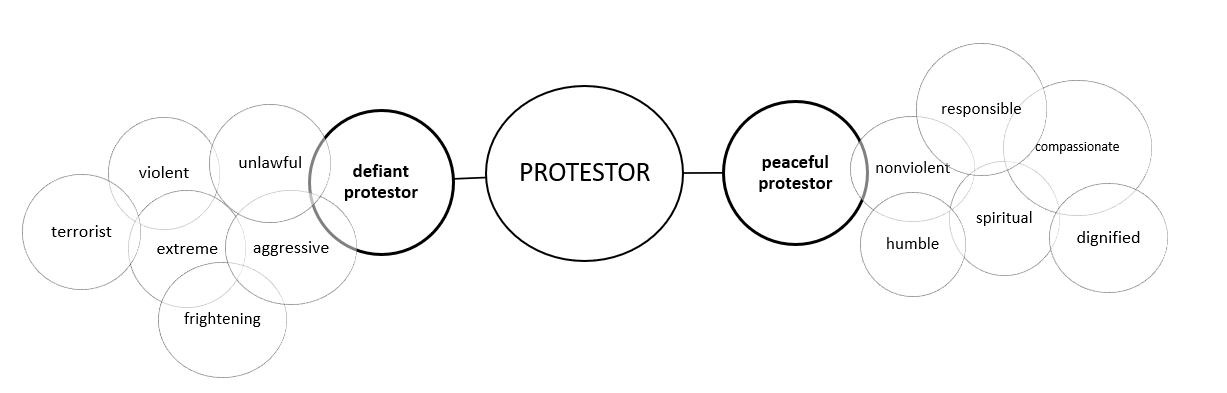
\includegraphics[width=14cm]{Figures/cluster.png}
\caption{Radial categories of \textsc{protester} with corresponding clusters of attributes}
\label{fig:figure1}
\end{figure}

\textbf{ICMs and Othering}

What is remarkable about the attributes in Table 4.2 and Figure 4.3, is the degree to which concepts on the opposing columns (or radial nodes) are opposites to each other. In short, the ICMs juxtapose. All Group A statements place protesters on the \textit{defiant protester} node, while all in Groups B and C place them on the \textit{peaceful} node. Moreover, the attributes on each side are not merely different variations, they are opposites. Here, we explore how this categorization is crucial to understanding the process of othering.

There is evidence to suggest dualistic thought patterns are hardwired into the human brain. According to \citeauthor{LeDoux1994}'s (\citeyear{LeDoux1994}) studies on the neurology of emotions, any information entering the central nervous system is unconsciously assigned a ``good'' or ``bad'' label \citep[31]{Wood2005}. Moreover, this choice is determined by the amygdala before further processing by the cortex.  At least when it comes to emotions and the unconscious, the tendency to categorize information in a dualistic manner seems deeply rooted in the human mind. However, the fact that information is unconsciously categorized by the amygdala does not imply there is no room for further cognitive processing. Further processing and modulating of sensory information is possible since ``the cerebral cortex can dialogue with the amygdala'' \citep[32]{Wood2005}. More sophisticated thinking that accounts for gradation and nuance depends precisely on this dialogue.   

Othering can be understood in terms of dualistic, emotional thought processes. At its essence, identifying another human as `other' is to create a polar dichotomy between that human and the `self'. As an unconscious, emotionally driven cognitive process, othering builds upon this polar diachotomy with what \citeauthor{Fedor2014a} (\citeyear{Fedor2014a}) calls ``antagonistic pairs.''        

\begin{quote}
The relation between me-the other one can be illustrated through a series of antagonistic pairs....similar-different; local-foreign; close-far; friend-enemy; normal-deviant; majority-minority. (322)   
\end{quote}

Considering the ICM used by Group A speakers to categorize \textsc{protester}, we can see antagonistic pairs being created through the discourse. Unlawful-lawful and orderly-disorderly are two examples. Local-foreign is also at play, as exemplified in the following statements:

\begin{footnotesize}
\begin{itemize}
\item[] \texttt{Unfortunately, a lot of times these things can be overwhelmed from outside groups.\newline 
\textit{-Senator Scott Martin}}
\newline
\item[] \texttt{There is an element there of people protesting who are frightening. It's time for them to go home. \newline 
\textit{-North Dakota Attorney General Wayne Stenehjem}}
\end{itemize}
\end{footnotesize} 

The portrayal of protesters as originating from outside the area is a discursive move that is consistent with the \textsc{protester} ICM. To describe the protesters as ``local'' or ``neighbours'' would be inconsistent with the other dichotomies that underpin the protesters as `other'. The phrase ``go home'' might be interpreted in a similar way. Or, one might consider another dichotomy as private-public, where ``home'' denotes the private sphere. This would expand the idea discussed in the socio-economic level, where Group A speakers present themselves as maintaining public order in the name of protecting the private sphere.

Othering manifests as stereotype when `in group' and `out group' dynamics come into play. `Self' and `other' takes on the dimension of `us' and `them'. Like the notion of the other, us/them identities are created through discourse. The preceding discussion gives examples of how ``out group'' status is assigned to protesters. In Group A, we can also see more subtle appeals to the in-group. For example, the repeated claim that protesters are a ``public safety issue'' creates an `in group' of law abiding citizens. Similarly, the claim that protesters ``make life difficult for everyone who lives and works in the area,'' is an `in group' of all local working people. Finally, when the Attorney General refers to a donation from the pipeline company Energy Transfer partners as ``a gift to the people of North Dakota,'' all people of the state are an `in group' vis-\`a-vis protesters who, despite also being citizens, have been cast as an `out group'.      

\textbf{Summary of the Cognitive Level}

By reading quotes from the corpus, one can quickly see that pipeline protesters are being portrayed using consistent language and concepts, particularly related to aggressive and unlawful behaviour. Not only do the various speakers in Group A refer to protesters in a consistent manner, but the language they use is often opposite to that of Groups B and C. While it is expected that Groups B and C would contrast with Group A, the extent to which pipeline proponents/opponents employ polar opposite concepts is noteworthy. 

The notion of Idealize Cognitive Models (ICM) is one way to understand how protesters are framed according to two opposing radial categories: \textit{defiant protester} and \textit{peaceful protester}. Attributes cluster around these radial nodes. The othering and stereotyping arises from this binary categorization of the concept \textsc{protester}. In other words, ICMs give us a framework for understanding the apparent stereotyping of protesters as a consequence of the way humans unconsciously categorize information.

\section{Summary \& Conclusions}

This chapter opened by highlighting the diverse perspectives surrounding infrastructure projects like the Dakota Access Pipeline (DAP). It was also pointed out that, due to the high profile nature of this project, the volume of communication is particularly large. If attempting to analyze the issue, the breadth of perspectives and communication artifacts presents a methodological challenge. In order to address this challenge, a multilevel approach using corpus data was employed. Specifically, quotations were extracted in order to break down the large volume of linguistic data into meaningful segments. Organizing the quotations into three groups (A, B, and C) made it possible to carry out a comparative analysis. The following is a summary of the analysis.

\begin{itemize}
  \item Keywords suggest dominant themes among proponents (Group A) to be security and law. Group A keywords also indicate possible negative portrayals of pipeline opponents. \textit{Protester} is the second most common keyword in this Group. Group B keywords also contain language related to public institutions and laws (e.g. \textit{right}, \textit{government}). Also, ecological-related terms appear in Group B (e.g. \textit{land}, \textit{water}). Group C has some overlap with B, but cultural terms are more apparent (e.g, \textit{sacred}, \textit{prayer}).
  
 \item In Group A, nature is referred to in the context of resources and management. Energy and infrastructure are discussed in terms of security and safety. An overarching discourse strategy in Group A is establishing and upholding legitimacy over resources and infrastructure. 
 
  \item In Group B, the natural environment is contested as a site of political/economic injustice. Power dynamics of resources and infrastructure are discussed. Group B can be seen as being in dialogue with Group A, insofar as an overarching discourse strategy is challenging the legitimacy of institutions to manage natural resources.
  
  \item In Group C, nature is a source of cultural identity. Statements refer to a holistic relationships between people, culture, and economy. Group C operates in an entirely different frame of meaning than both A and B. 
  
  \item In Group A, we notice that identifiable sub-groups of the population are not mentioned. Protesters and opponents are anonymized and disassociated from society. Group A statements suggest that othering involves a stripping away of culture.
  
  \item Clusters of concepts used in Group A show how othering and stereotyping might result from the way humans categorize information. The negative associations with pipeline opponents can be understood in terms of Idealized Cognitive Models (ICMs) of the concept \textsc{protester}.

\end{itemize}

One could make the case that the above results are merely consistent with the way in which groups were selected. For instance, one would expect Group A to portray protesters in a negative light, Group C would contain cultural keywords, and so on. However, the main conclusions from this analysis arise from the comparison of communication between the groups, not each group in isolation. By contrasting Groups A and B with Group C, we get clearer insight into what constitutes cultural discourse. 

In Chapter 2, we discussed the nuanced and fuzzy distinction between the cultural and socio-economic levels. The former was associated with \textit{Kultur} as an inner spirit of human experience; the latter with \textit{Zivilization} with the outer shell. In this light, one might consider Groups A and B as having to do with \textit{Zivilization}. The groups dealt with institutions, administrative systems, and corporate structures that encompass all a society. Group C, by contrast, was the source of identity and expression of inner (cultural) meanings within the society.    